%iffalse
\let\negmedspace\undefined
\let\negthickspace\undefined
\documentclass[journal,15pt,onecolumn]{IEEEtran}
\usepackage{cite}
\usepackage{amsmath,amssymb,amsfonts,amsthm}
\usepackage{algorithmic}

\usepackage{textcomp}
\usepackage[table,xcdraw]{xcolor}
\usepackage{txfonts}
\usepackage{listings}
\usepackage{enumitem}
\usepackage{mathtools}
\usepackage{gensymb}
\usepackage{enumitem}
\usepackage{comment}
\usepackage[breaklinks=true]{hyperref}
\usepackage{tkz-euclide} 
\usepackage{gvv}                                        
%\def\inputGnumericTable{}
\usepackage[utf8]{inputenc} 
\usepackage{xparse}
\usepackage{color}
\usepackage{graphicx}
\usepackage{array}                                            
\usepackage{longtable}                                       
\usepackage{calc}                                             
\usepackage{multirow}
\usepackage{multicol}
\usepackage{hhline}                                           
\usepackage{ifthen}                                           
\usepackage{lscape}
\usepackage{tabularx}
\usepackage{array}
\usepackage{float}
\newtheorem{theorem}{Theorem}[section]
\newtheorem{problem}{Problem}
\newtheorem{proposition}{Proposition}[section]
\newtheorem{lemma}{Lemma}[section]
\newtheorem{corollary}[theorem]{Corollary}
\newtheorem{example}{Example}[section]
\newtheorem{definition}[problem]{Definition}
\newcommand{\BEQA}{\begin{eqnarfnray}}
\newcommand{\EEQA}{\end{eqnarray}}
%\newcommand{\define}{\stackrel{\triangle}{=}}
\theoremstyle{remark}
%\newtheorem{rem}{Remark}
% Marks the beginning of the document

\begin{document}


\title{gate 2}
\author{AI25btech11037 - STALIN}
\maketitle
\renewcommand{\thefigure}{\theenumi}
\renewcommand{\thetable}{\theenumi}




\begin{enumerate}




\item 
If '$\rightarrow$' denotes increasing order of intensity, then the meaning of the words 

$[ \text{dry} \;\to\; \text{arid} \;\to\; \text{parched} ]$    is analogous to     $[ \text{diet} \;\to\; \text{fast} \;\to\; \_\_\_\_\_\_ ]$.
 
Which one of the given options is appropriate to fill the blank?  \hfill \textbf{ (GATE NM 2024)}

\begin{enumerate}
\item (i) starve
\item (i) reject
\item (i) feast
\item (i) deny
\end{enumerate}


\item 
If two distinct non-zero real variables $x$ and $y$ are such that $(x+y)$ is proportional to $(x-y)$ then the value of $\dfrac{x}{y}$  \hfill \textbf{ (GATE NM 2024)}

\begin{enumerate}
\item (i) depends on $xy$
\item (i) depends only on $x$ and not on $y$
\item (i) depends only on $y$ and not on $x$
\item (i) is a constant
\end{enumerate}

 \item  Consider the following sample of numbers:  
    \[ 9, \; 18, \; 11, \; 14, \; 15, \; 17, \; 10, \; 69, \; 11, \; 13 \]  
    The median of the sample is\hfill \textbf{ (GATE NM 2024)}
    \begin{enumerate}
        \item (i) 13.5
        \item (i) 14
        \item (i) 11
        \item (i) 18.7
    \end{enumerate}
    
    
    \item  The number of coins of  Rs 1, Rs 5, and Rs 10 denominations that a person has are in the ratio $5:3:13$.  
    Of the total amount, the percentage of money in Rs 5 coins is\hfill \textbf{ (GATE NM 2024)}
    
    \begin{enumerate}
        \item (i) 21\%
        \item (i) $14 \dfrac{2}{7}\%$
        \item (i) 10\%
        \item (i) 30\%
    \end{enumerate}
    

    \item   For positive non-zero real variables $p$ and $q$, if
    
     $$  \log \left(p^{2} + q^{2}\right) = \log p + \log q + 2 \log 3 $$
    then, the value of $$ \frac{p^{4} + q^{4}}{p^{2}q^{2}}$$\hfill \textbf{ (GATE NM 2024)}
    
    is
    \begin{enumerate}
        \item (i) 79
        \item (i) 81
        \item (i) 9
        \item (i) 83
    \end{enumerate}


\item  In the given text, the blanks are numbered (i)--(iv). Select the best match for all the blanks.

  Steve was advised to keep his head \rule{1cm}{0.15mm} (i) before heading \rule{1cm}{0.15mm} (ii) to bat; for, while he had a head \rule{1cm}{0.15mm} (iii) batting, he could only do so with a cool head \rule{1cm}{0.15mm} (iv) his shoulders.\hfill \textbf{ (GATE NM 2024)}

    \begin{enumerate}
        \item (i)  down \quad(ii) down \quad (iii) on \quad (iv) for
        \item (i)  on \quad(ii) down \quad (iii) for \quad  (iv) on
        \item (i)  down \quad(ii) out \quad (iii) for \quad (iv) on
        \item (i)  on \quad(ii) out \quad (iii) on \quad  (iv) for
    \end{enumerate}



\item  A rectangular paper sheet of dimensions $54 \, \text{cm} \times 4 \, \text{cm}$ is taken. 
  The two longer edges of the sheet are joined together to create a cylindrical tube. 
  A cube whose surface area is equal to the area of the sheet is also taken. 
  
  Then, the ratio of the volume of the cylindrical tube to the volume of the cube is\hfill \textbf{ (GATE NM 2024)}\hfill \textbf{ (GATE NM 2024)}

  \begin{enumerate}
    \item  $\tfrac{1}{\pi}$
    \item  $\tfrac{2}{\pi}$
    \item  $\tfrac{3}{\pi}$
    \item  $\tfrac{4}{\pi}$
  \end{enumerate}

\item The pie chart presents the percentage contribution of different macronutrients 
  to a typical $2000 \, \text{kcal}$ diet of a person.\hfill \textbf{ (GATE NM 2024)}


\begin{figure}[h!]
        \centering
        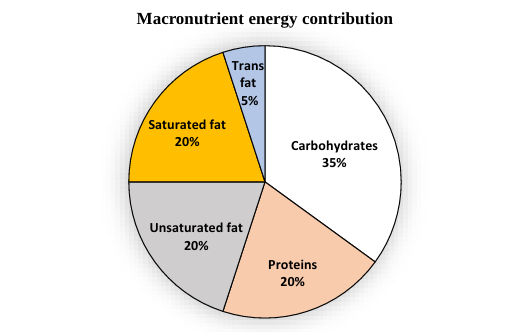
\includegraphics[width=0.7\linewidth]{figures.tex/Screenshot 2025-08-20 122315.png}
        \caption{ Caption}
        \label{fig:placeholder}
    \end{figure}
       

\item 
  The typical energy density (kcal/g) of these macronutrients is given in the table.



The total fat (all three types), in grams, this person consumes is:\hfill \textbf{ (GATE NM 2024)}

\begin{figure}[h!]
    \centering
    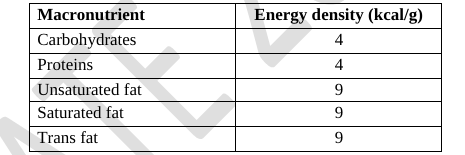
\includegraphics[width=0.9\linewidth]{figures.tex/Screenshot 2025-08-20 123147.png}
    \caption{Caption}
    \label{fig:placeholder}
\end{figure}
\begin{enumerate}
\item 44.4
\item 77.8 
\item 100
\item 3,600
\end{enumerate}



\item 
A rectangular paper of 20 cm  8 cm is folded 3 times. Each fold is made along the line of symmetry, which is perpendicular to its long edge. The perimeter of the final folded sheet (in cm) is:\hfill \textbf{ (GATE NM 2024)}

\begin{enumerate}
    \item 18
    \item 24
    \item 20
    \item 21
\end{enumerate}

\item 
The least number of squares to be added in the figure to make AB a line of symmetry is:\hfill \textbf{ (GATE NM 2024)}

\begin{figure} [h!]
    \centering
    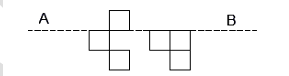
\includegraphics[width=0.5\linewidth]{figures.tex/Screenshot 2025-08-20 150832.png}
    \caption{Caption}
    \label{fig:placeholder}
\end{figure}


\begin{enumerate}
    \item 6
    \item 4
    \item 5
    \item 7
\end{enumerate}



    \item
    The value of the contour integral 
    $
    \oint \frac{dz}{2z - z^2}
    $
    along the circle \(|z| = 1\), oriented in the counterclockwise sense is:\hfill \textbf{ (GATE NM 2024)}
    
    \begin{enumerate}
        \item $ \pi i $
        \item $ 0 $
        \item $ 2\pi i $
        \item $ 4\pi i $
    \end{enumerate}

    \item 
    The tangent plane to the surface $ x^2 + y^2 + z = 9 $ at the point $ (1, 2, 4) $ is\hfill \textbf{ (GATE NM 2024)}
    
    \begin{enumerate}
        \item $ 2x + 4y + z = 14 $
        \item $ 4x + 2y + z = 12 $
        \item $ x + 4y + 2z = 17 $
        \item $ 4x + y + 2z = 14 $
    \end{enumerate}

 \item The value of the line integral 
    $ \oint x^2\, dx + 2x\, dy $
    along the ellipse $ 4x^2 + y^2 = 4 $, oriented in the counterclockwise sense is:\hfill \textbf{ (GATE NM 2024)}

    \begin{enumerate}
        \item $\pi$
        \item $2\pi$
        \item $4\pi$
        \item $8\pi$
    \end{enumerate}

    \item The system of linear equations \\
    $
    \begin{aligned}
        x + 2y + 3z &= 4 \\
        2x - y - 2z &= a^2 \\
        -x - 7y - 11z &= a
    \end{aligned}
    $ \\
    has a solution if the values of $a$ are:

    \begin{enumerate}
        \item $-1$ and $5$
        \item $-2$ and $3$
        \item $-5$ and $1$
        \item $-3$ and $4$
    \end{enumerate}

 \item A ship with a standard right-handed coordinate system has positive $x$, $y$, and $z$ axes respectively pointing towards bow, starboard and down as shown in the figure. If the ship takes a starboard turn, then the drift angle, sway velocity and the heel angle of the ship for a steady yaw rate respectively are:\hfill \textbf{ (GATE NM 2024)}

\begin{figure}[h!]
    \centering
    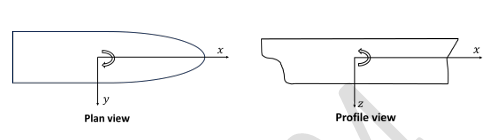
\includegraphics[width=0.8\linewidth]{figures.tex/Screenshot 2025-08-20 152911.png}
    \caption{Caption}
    \label{fig:placeholder}
\end{figure}

\begin{enumerate}
        \item positive, negative and positive
        \item negative, positive and positive
        \item negative, positive and negative
        \item positive, negative and negative
    \end{enumerate}

  \item A ship with controls fixed, is modeled as a two degrees of freedom system. For the linear maneuvering equations of motion for coupled sway and yaw, if the derived eigenvalues are real and negative, then the ship must possess:\hfill \textbf{ (GATE NM 2024)}

    \begin{enumerate}
        \item positional motion stability
        \item directional stability
        \item straight line stability
        \item both directional and positional motion stabilities
    \end{enumerate}

    \item Which one of the following cooling systems is used in large marine diesel engines?\hfill \textbf{ (GATE NM 2024)}

    \begin{enumerate}
        \item Thermosyphon
        \item Forced coolant circulation
        \item Evaporative
        \item Air circulation
    \end{enumerate}

 \item Which one of the following reduces the ratio of vibratory response amplitude to the forcing amplitude, in large stationary engine shaft design?\hfill \textbf{ (GATE NM 2024)}

    \begin{enumerate}
        \item Reduction in axial vibrations of the rotating shaft
        \item Increase in the fundamental frequency of the rotating shaft
        \item Decrease in the rotational speed of shaft
        \item Operating the shaft at a speed exceeding the critical speed
    \end{enumerate}


 \item
 The GZ curve for a stable ship is shown in the figure, where P is a point of inflection on the curve. Match the labels in \textbf{Column 1} with the corresponding descriptions in \textbf{Column 2}.\hfill \textbf{ (GATE NM 2024)}\hfill \textbf{ (GATE NM 2024)}

\begin{figure} [h!]
    \centering
    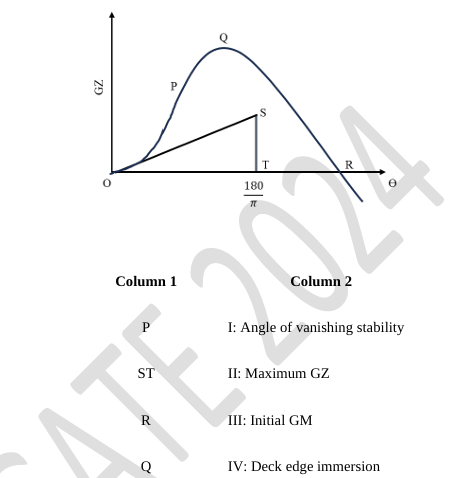
\includegraphics[width=0.8\linewidth]{figures.tex/Screenshot 2025-08-20 153735.png}
    \caption{Caption}
    \label{fig:placeholder}
\end{figure}

  \begin{enumerate}
    \item R - I; Q - II; ST - III; P - IV
    \item P - I; Q - II; ST - III; R - IV
    \item ST - I; Q - II; R - III; P - IV
    \item R - I; Q - II; P - III; ST - IV
  \end{enumerate}


  \item
  Consider an initially perfectly straight elastic column with pinned supports at both ends. If E is the Young’s modulus of the material, L is the length of the column between the supports, and . I is the least moment of inertia of the constant cross-sectional area of the column, then the Euler load is given by .\hfill \textbf{ (GATE NM 2024)}

  \begin{enumerate}
    \item $\dfrac{\pi^2 EI}{L^2}$
    \item $\dfrac{\pi^2 EI}{4L^2}$
    \item $\dfrac{\pi^2 EI}{\sqrt{2}L^2}$
    \item $\dfrac{2\pi^2 EI}{L^2}$
  \end{enumerate}

  \item For a plane strain problem in the $x$-$y$ plane, it is necessary that\hfill \textbf{ (GATE NM 2024)}

  \begin{enumerate}
    \item normal stress $\sigma_z$ is zero
    \item normal strain $\varepsilon_z$ is zero
    \item both the normal stresses $\sigma_x$ and $\sigma_y$ are zero
    \item shear strain $\gamma_{xy}$ is equal to $\dfrac{\varepsilon_x - \varepsilon_y}{2}$
  \end{enumerate}

 \item How many independent material constants in solids are required to define isotropic materials?\hfill \textbf{ (GATE NM 2024)}

  \begin{enumerate}
    \item 2
    \item 3
    \item 9
    \item 21
  \end{enumerate}



\item Which one of the following is the mass conservation equation?\hfill \textbf{ (GATE NM 2024)}

  \begin{enumerate}
    \item 
    $
    \frac{D}{Dt} \iiint_V \rho \, \vec{v} \cdot \hat{n} \, dV = 0
    $
    \item 
    $
    \frac{\partial}{\partial t} \iiint_V \rho dV = 0
    $
    \item 
    $
    -\frac{\partial}{\partial t} \iiint_V \rho dV = \iint_S \rho \vec{v} \cdot \hat{n} \, ds
    $
    \item 
    $
    -\frac{D}{Dt} \iiint_V \rho dV = \iint_S \rho \vec{v} \cdot \hat{n} \, ds
    $
  \end{enumerate}

 \item Identify the type of flow from the time series plots of instantaneous fluid velocity (u) at a point.\hfill \textbf{ (GATE NM 2024)}

\begin{figure}[h!]
    \centering
    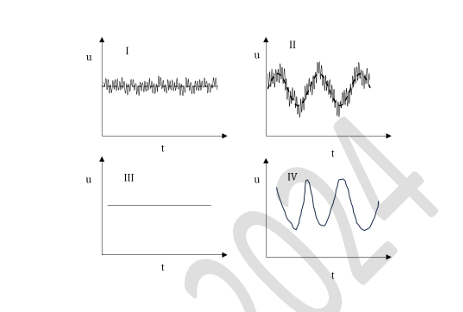
\includegraphics[width=1.0\linewidth]{figures.tex/Screenshot 2025-08-20 155122.png}
    \caption{Caption}
    \label{fig:placeholder}
\end{figure}



\begin{enumerate}
    \item I - unsteady turbulent flow; II - steady turbulent flow; 
    III - steady laminar flow; IV - unsteady laminar flow

    \item I - steady turbulent flow; II - unsteady turbulent flow; 
    III - unsteady laminar flow; IV - steady laminar flow

    \item I - steady turbulent flow; II - unsteady turbulent flow; 
    III - steady laminar flow; IV - unsteady laminar flow

    \item I - steady turbulent flow; II - unsteady laminar flow; 
    III - unsteady turbulent flow; IV - steady laminar flow
\end{enumerate}


\item
Which of the following hull distortion(s) is/are resisted by a ship’s transverse bulkhead?\hfill \textbf{ (GATE NM 2024)}
    \begin{enumerate}
    
        \item Racking
        \item Torsion
        \item Longitudinal bending
        \item Horizontal bending
    \end{enumerate}

    \item
    Which of the following boiler(s) is/are \textbf{NOT} used in a nuclear propulsion system for ships?\hfill \textbf{ (GATE NM 2024)}
    
    \begin{enumerate}
        \item Water tube boiler
        \item Cochran boiler
        \item Double evaporation boiler
        \item Boiled water reactor boiler
    \end{enumerate}


\item
Which of the following statement(s) is/are correct about strip theory?\hfill \textbf{ (GATE NM 2024)}
    \begin{enumerate}
        \item It can be used to calculate the surge added mass
        \item It is a two-dimensional theory
        \item It can be used to calculate the pitch added mass
        \item It can be used to calculate the coupled sway, roll and yaw added mass
    \end{enumerate}

    \item
    Consider an ideal Rankine cycle as shown in the figure, where $T$ and $S$ represent the temperature and entropy respectively. 
    The overall efficiency of the cycle can be improved \hfill \textbf{ (GATE NM 2024)}

\begin{figure} [h!]
    \centering
    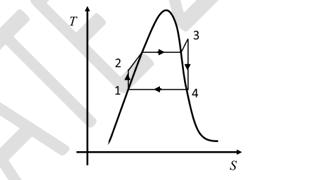
\includegraphics[width=0.8\linewidth]{figures.tex/Screenshot 2025-08-21 111305.png}
    \caption{Caption}
    \label{fig:placeholder}
\end{figure}




 \item Consider an ideal Rankine cycle as shown in the figure, where $T$ and $S$ represent the temperature and entropy respectively. 
    The overall efficiency of the cycle can be improved by\hfill \textbf{ (GATE NM 2024)}
    \begin{enumerate}
        \item increasing the pressure at which heat is added
        \item decreasing the pressure at which heat is rejected
        \item employing an intercooler
        \item superheating the steam
    \end{enumerate}



 \item Which of the following statement(s) is/are correct for a thermodynamic closed system?\hfill \textbf{ (GATE NM 2024)}
    \begin{enumerate}
        \item The entropy change is positive for a reversible adiabatic process
        \item The entropy change is positive for a reversible cycle
        \item The entropy change is positive for a reversible isothermal heat addition process
        \item The entropy change is negative for a reversible isothermal heat rejection process
    \end{enumerate}

    \item The arc length of the one arch of the cycloid given by $x = t - \sin t$ and $y = 1 - \cos t$ is \_\_\_\_\_\_.\hfill \textbf{ (GATE NM 2024)}
    
    \item A 10 m long pipe with inlet and outlet diameters of 40 cm and 20 cm respectively, 
    is carrying an incompressible fluid with a flow rate of $0.04 \, \text{m}^3/\text{s}$. 
    The ratio of the velocity at the outlet to that at the inlet is \_\_\_\_\_ (rounded off to one decimal place).\hfill \textbf{ (GATE NM 2024)}



 \item An 80 m long barge with rectangular cross-section of 12 m beam and 4 m draft floats at even keel. 
    The transverse metacenter (KM) above the keel is \_\_\_\_\_ m.\hfill \textbf{ (GATE NM 2024)}

    \item A 100 m long ship has a cruising speed of 25 knots. 
    A geometrically similar model of 4 m length is used for resistance prediction in a towing tank. 
    The corresponding speed of the model is \_\_\_\_\_\_\_\_\_\_\_ knots.\hfill \textbf{ (GATE NM 2024)}

    \item A cube-shaped pontoon with 200 tonnes of mass placed on it, floats with a freeboard of 1 m in fresh water. 
    When the mass is removed, the pontoon floats with a freeboard of 3 m. 
    The length of the pontoon is \_\_\_\_\_ m (rounded off to two decimal places).\hfill \textbf{ (GATE NM 2024)}


 \item Consider a fluid between two horizontal parallel flat plates 5 mm apart as shown in the figure. 
    The top plate of dimensions $0.5 \, \text{m} \times 2 \, \text{m}$ is towed with an applied horizontal force $F$ of $0.01 \, \text{N}$, 
    while the infinitely long bottom plate is kept fixed. 
    The horizontal velocity profile between the plates is assumed to be linear. 
    If the dynamic viscosity $(\mu)$ of the fluid is $0.89 \times 10^{-3} \, \text{N$\cdot$s}/\text{m}^2$, 
    then the towing velocity of the top plate is \_\_\_\_\_ m/s (rounded off to three decimal places).\hfill \textbf{ (GATE NM 2024)}


\begin{figure}[h!]
    \centering
    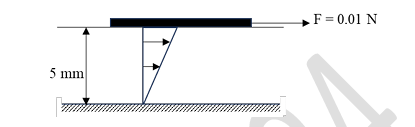
\includegraphics[width=0.8\linewidth]{figures.tex/Screenshot 2025-08-21 112416.png}
    \caption{Caption}
    \label{fig:placeholder}
\end{figure}



 \item Consider the matrices 
    $ M = \begin{pmatrix} 2 & 1 \\ 0 & 2 \end{pmatrix}, \quad 
    N = \begin{pmatrix} 1 & 0 & 0 \\ 1 & 2 & 0 \\ 1 & 1 & 0 \end{pmatrix}. 
    $
    Which one of the following is true?\hfill \textbf{ (GATE NM 2024)}
    \begin{enumerate}
        \item $M$ is not diagonalizable but $N$ is diagonalizable
        \item Both $M$ and $N$ are not diagonalizable
        \item Both $M$ and $N$ are diagonalizable
        \item $M$ is diagonalizable but $N$ is not diagonalizable
    \end{enumerate}

\item A simply supported beam is subjected to a concentrated moment $M$ at the mid span as shown in the figure. 
    The magnitude of the bending moment at a distance of $L/4$ from the left support A is equal to \_\_\_\_\_.\hfill \textbf{ (GATE NM 2024)}




\begin{figure}[h!]
    \centering
    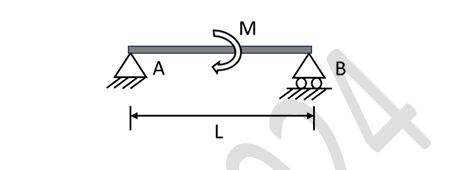
\includegraphics[width=0.8\linewidth]{figures.tex/Screenshot 2025-08-21 112803.png}
    \caption{Caption}
    \label{fig:placeholder}
\end{figure}


  \item A simply supported beam is subjected to a concentrated moment $M$ at the mid span as shown in the figure. 
    The magnitude of the bending moment at a distance of $\tfrac{L}{4}$ from the left support $A$ is equal to \_\_\_\_\_.\hfill \textbf{ (GATE NM 2024)}

\item Consider a two-dimensional ship section as shown in the figure. 
    About the point $O$, let the sway added mass components be $a_{22}$ and $a_{24}$ 
    and roll added moment of inertia be $a_{44}$. 
    The clockwise roll angle is considered positive. 
    The roll added mass due to roll, about $P$ which is at a distance $z_P$ above $O$ is given by\hfill \textbf{ (GATE NM 2024)}

\begin{figure}[h!]
    \centering
    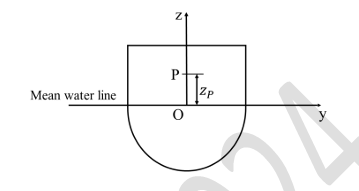
\includegraphics[width=0.8\linewidth]{figures.tex/Screenshot 2025-08-21 113134.png}
    \caption{Caption}
    \label{fig:placeholder}
\end{figure}

\begin{enumerate}

    \item $a_{44} - a_{24} z_{P}$
    \item $a_{44} - a_{22} z_{P} - a_{24} z_{P}$
    \item $a_{44} - a_{22} z_{P} + a_{24} z_{P}$
    \item $a_{22} + a_{24} + a_{44}$
\end{enumerate}
 \item
 A ship with a displacement of 10000 tonnes has the center of gravity at 4\,m above the keel and 1.5\,m forward of midship. If 2000 tonnes of cargo is placed at 10\,m above the keel and 1.5\,m aft of midship, then the new position of the center of gravity is\hfill \textbf{ (GATE NM 2024)}
 
    \begin{enumerate}
        \item 5\,m above the keel and 1\,m aft of midship
        \item 6\,m above the keel and 1\,m forward of midship
        \item 6\,m above the keel and 1\,m aft of midship
        \item 5\,m above the keel and 1\,m forward of midship
    \end{enumerate}
    
    \item
    The waterplane area of a ship floating in sea water is $2000\,\text{m}^2$. The density of seawater is $1025\,\text{kg}/\text{m}^3$. If a mass of $246$ tonnes is added to the ship, then the TPC (Tonnes Per Centimeter immersion) and increase in draft (in cm) respectively are\hfill \textbf{ (GATE NM 2024)}
    
    \begin{enumerate}
        \item $20.50$ and $12$
        \item $20$ and $12.3$
        \item $20.50$ and $24$
        \item $10.25$ and $24.6$
    \end{enumerate}



    \item
    The open water characteristics of a propeller is shown in the figure. Match the labels in \textbf{Column 1} with the corresponding descriptions in \textbf{Column 2}\hfill \textbf{ (GATE NM 2024)}
    
\begin{figure}[h!]
    \centering
    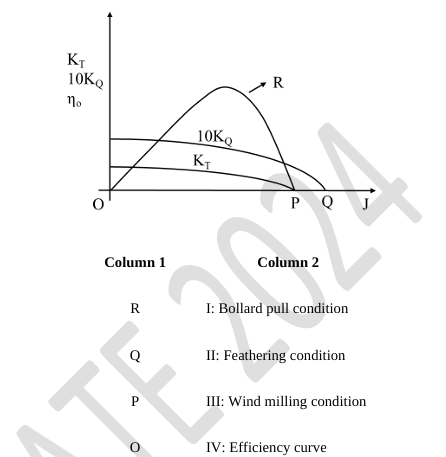
\includegraphics[width=0.5\linewidth]{figures.tex/Screenshot 2025-08-21 160411.png}
    \caption{Caption}
    \label{fig:placeholder}
\end{figure}


\begin{enumerate}
    \item $O - I; P - II; Q - III; R - IV$
    \item $O - I; Q - II; P - III; R - IV$
    \item $O - I; R - II; Q - III; P - IV$
    \item $P - I; Q - II; O - III; R - IV$
\end{enumerate}

\begin{figure}[h!]
    \centering
    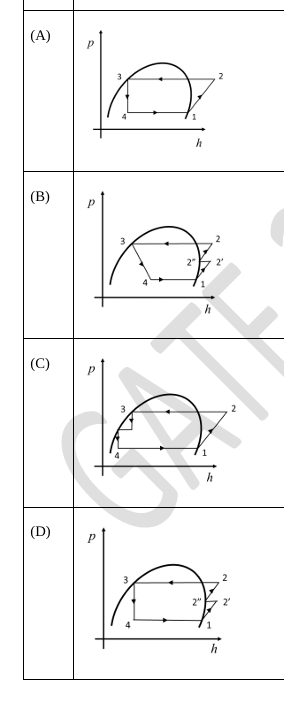
\includegraphics[width=0.5\linewidth]{figures.tex/Screenshot 2025-08-21 161434.png}
    \caption{Caption}
    \label{fig:placeholder}
\end{figure}

\item A steel deck plate of a tanker is supported by two longitudinal stiffeners as shown in the figure. The width of the plate is $a$ and its length is $5$ times the width. Assume that the long edge is simply supported, and the short edge is free. The plate is loaded by a distributed pressure, $p = p_0 \sin \left(\frac{\pi x}{a}\right)$, where $p_0$ is the pressure at $y = a/2$. The flexural rigidity of the plate is $D$. The plate equation is given by\hfill \textbf{ (GATE NM 2024)}

\begin{figure}[h!]
    \centering
    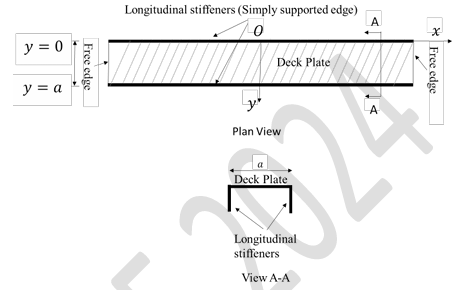
\includegraphics[width=0.5\linewidth]{figures.tex/Screenshot 2025-08-21 161935.png}
    \caption{Caption}
    \label{fig:placeholder}
\end{figure}

\begin{enumerate}
    \item $\dfrac{\partial^4 w}{\partial y^4} = \dfrac{p_0}{D} \sin \left(\dfrac{\pi y}{a}\right)$
    \item $\dfrac{\partial^2 w}{\partial x^2} = \dfrac{p_0}{D} \sin \left(\dfrac{\pi y}{a}\right)$
    \item $\dfrac{\partial^2 w}{\partial y^2} = \dfrac{p_0}{D} \sin \left(\dfrac{\pi y}{a}\right)$
    \item $\dfrac{\partial^4 w}{\partial x^4} = \dfrac{p_0}{D} \sin \left(\dfrac{\pi y}{a}\right)$
\end{enumerate}

\item Which one of the following psychrometric processes is represented by the line $1$-$2$ in the figure?\hfill \textbf{ (GATE NM 2024)}


\begin{figure}
    \centering
    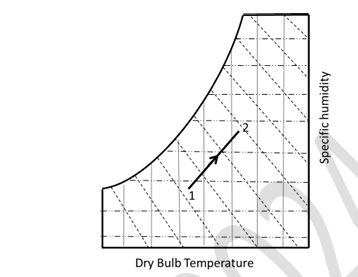
\includegraphics[width=0.5\linewidth]{figures.tex/Screenshot 2025-08-22 145453.png}
    \caption{Caption}
    \label{fig:placeholder}
\end{figure}


\begin{enumerate}
    \item Cooling and humidification
    \item Cooling and dehumidification
    \item Heating and humidification
    \item Heating and dehumidification
\end{enumerate}

\item
Consider model testing where $\lambda$ is the prototype to model length scale ratio. 
    Let $\nu_p$ and $\nu_m$ denote the corresponding fluid kinematic viscosities. 
    If Froude and Reynolds similarities are maintained between the prototype and model, 
    then which one of the following is correct?\hfill \textbf{ (GATE NM 2024)}
    
    \begin{enumerate}
        \item $\nu_m = \lambda^{-3/2} \nu_p$
        \item $\nu_m = \lambda^{3/2} \nu_p$
        \item $\nu_m = \lambda^{2/3} \nu_p$
        \item $\nu_m = \lambda^{-2/3} \nu_p$
    \end{enumerate}
    
 \item
 uniform flow, a point source of strength $+\sigma$ at $(a,0)$ and a point sink of
  strength $-\sigma$ at $(-a,0)$ are shown in the figure. The velocity potential $\phi$
  resulting from the superposition of these flow fields is given by\hfill \textbf{ (GATE NM 2024)}

\begin{figure}
    \centering
    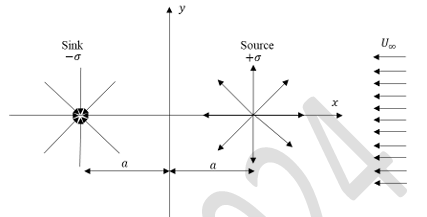
\includegraphics[width=0.5\linewidth]{figures.tex/Screenshot 2025-08-22 150107.png}
    \caption{Caption}
    \label{fig:placeholder}
\end{figure}
  
  \begin{enumerate}
    \item $\phi = -U_{\infty} x \;+\; \dfrac{\sigma}{2\pi}\ln\!\sqrt{(x+a)^2+y^2}
                \;-\; \dfrac{\sigma}{2\pi}\ln\!\sqrt{(x-a)^2+y^2}$
    \item $\phi = -U_{\infty} x \;+\; \dfrac{\sigma}{2\pi}\ln\!\sqrt{(x-a)^2+y^2}
                \;-\; \dfrac{\sigma}{2\pi}\ln\!\sqrt{(x+a)^2+y^2}$
    \item $\phi = \;\;\, U_{\infty} x \;+\; \dfrac{\sigma}{2\pi}\ln\!\sqrt{(x-a)^2+y^2}
                \;-\; \dfrac{\sigma}{2\pi}\ln\!\sqrt{(x+a)^2+y^2}$
    \item $\phi = \;\;\, U_{\infty} x \;+\; \dfrac{\sigma}{2\pi}\ln\!\sqrt{(x+a)^2+y^2}
                \;-\; \dfrac{\sigma}{2\pi}\ln\!\sqrt{(x-a)^2+y^2}$
  \end{enumerate}



 \item
 In the solution of statically indeterminate problems, Castigliano’s second theorem employs the\hfill \textbf{ (GATE NM 2024)}
 
  \begin{enumerate}
    \item principle of virtual work
    \item virtual displacement method
    \item virtual force method
    \item principle of least work
  \end{enumerate}

  \item
  Consider the function $f(x,y)=x^{4}+y^{4}-4xy+1$. Which of the following is/are correct?\hfill \textbf{ (GATE NM 2024)}
  
  \begin{enumerate}
    \item The minimum value of $f$ occurs at $(0,0)$
    \item The point $(0,0)$ is a point of inflection
    \item $f$ has three critical points
    \item The minimum value of $f$ is $-1$
  \end{enumerate}

\item
Consider the $2\pi$–periodic function defined by
  $
    f(x)=
    \begin{cases}
      -1 & \text{if } -\pi < x \le 0,\\[4pt]
       1 & \text{if } 0 < x \le \pi.
    \end{cases}
  $
  
  Which of the following is/are correct about its Fourier series expansion,
  $\dfrac{a_0}{2}+\sum_{n=1}^{\infty}a_n\cos nx + b_n\sin nx$?\hfill \textbf{ (GATE NM 2024)}
  
  \begin{enumerate}
    \item $a_n=\dfrac{1}{n}\;\forall\; n=1,2,\ldots$
    \item $a_0=0$
    \item $b_n=\dfrac{4}{n\pi}$ if $n$ is odd
    \item $b_n=-\dfrac{4}{n\pi}$ if $n$ is even
  \end{enumerate}




\item 
Consider the following momentum equation. Let A, B and C denote the first, second
  and third term on the left-hand side respectively, and D, and E denote the first and
  second term on the right-hand side respectively. Which of the following statement(s)
  is/are correct?
  $
    \rho\left[\frac{\partial \mathbf{V}}{\partial t}
    + \nabla\!\left(\frac{|\mathbf{V}|^{2}}{2}\right)
    + (\nabla\times\mathbf{V})\times\mathbf{V}\right]
    = -\nabla\!\left(P+\rho g z\right) + \mu\nabla^{2}\mathbf{V}
  $\hfill \textbf{ (GATE NM 2024)}
  \begin{enumerate}
    \item If terms A, C and E vanish, then the flow is irrotational.
    \item If term A vanishes, then the flow is steady.
    \item If term D vanishes, then it leads to the Euler's equation.
    \item If terms A, B, C and E vanish, then it leads to the hydrostatic equation.
  \end{enumerate}



\item
Consider the flow past a curved wall as shown in the figure. Which of the
  following statement(s) is/are correct?\hfill \textbf{ (GATE NM 2024)}
 

\begin{figure}
    \centering
    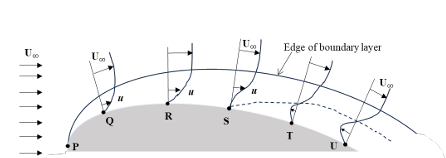
\includegraphics[width=0.5\linewidth]{figures.tex/Screenshot 2025-08-22 151031.png}
    \caption{Caption}
    \label{fig:placeholder}
\end{figure}

\item
Consider the flow past a curved wall as shown in the figure. 
  Which of the following statement(s) is/are correct?\hfill \textbf{ (GATE NM 2024)}
  
\begin{enumerate}
    \item[(A)] P is the separation point.
    \item[(B)] Between T and U, the pressure gradient in the streamwise direction at the wall is positive.
    \item[(C)] U is the stagnation point.
    \item[(D)] Between T and U, the streamwise-velocity gradient in the normal direction at the wall is negative.
\end{enumerate}

\item 
If $X$ is a Poisson random variable with mean $\mu = 1$, then the conditional probability of the event $\{X \geq 2\}$ given that the event $\{X \geq 4\}$ has occurred, is \_\_\_\_ (rounded off to two decimal places).\hfill \textbf{ (GATE NM 2024)}

\item 
The value of the triple integral 
$
\iiint (6x^2 + y^2) \, dx \, dy \, dz
$
over the region given by $-1 \leq x \leq 1,\; 3 \leq y \leq 5,\; 0 \leq z \leq 1$, is \_\_\_\_.\hfill \textbf{ (GATE NM 2024)}

\item 
A 4-cylinder, 4-stroke diesel engine operating at $3000 \,\text{rpm}$ has a compression ratio of $21$ and cut-off ratio of $2.5$. The temperature inside the head at the beginning of compression is $300 \,\text{K}$. The efficiency of an air standard diesel cycle is given by 
$
\eta = 1 - \frac{1}{r^{\gamma - 1}} \cdot \frac{r_c^\gamma - 1}{\gamma (r_c - 1)}.
$
Assume the working fluid as air with a mass flow rate of $0.05 \,\text{kg/s}$, $\gamma = 1.4$, and $C_v = 1.004 \,\text{kJ/kgK}$.

The power output of the engine is \_\_\_\_ kW (rounded off to the nearest integer).\hfill \textbf{ (GATE NM 2024)}

\item 
A ship travelling in head seas experiences a bending moment of $200 \,\text{MN-m}$. The ship’s cross-section is assumed to be a box girder of $20 \,\text{m}$ beam and $10 \,\text{m}$ depth, with a $10 \,\text{mm}$ plate thickness. The maximum bending stress is \_\_\_\_ MPa (rounded off to the nearest integer).\hfill \textbf{ (GATE NM 2024)}

\item 
A single degree of freedom system has a mass, stiffness and damping of $200 \,\text{kg}$, $20 \,\text{MN/m}$ and $8 \,\text{kNs/m}$ respectively. For a forced oscillating system, if the exciting frequency $\omega$ is equal to the undamped natural frequency, then the dynamic magnification factor is \_\_\_\_ (rounded off to three decimal places).\hfill \textbf{ (GATE NM 2024)}

\item 
The wave spectrum and the ship heave Response Amplitude Operator (RAO) are shown in the figure. The variance of the heave motion is \_\_\_\_ (rounded off to two decimal places).\hfill \textbf{ (GATE NM 2024)}

\begin{figure} [h!]
    \centering
    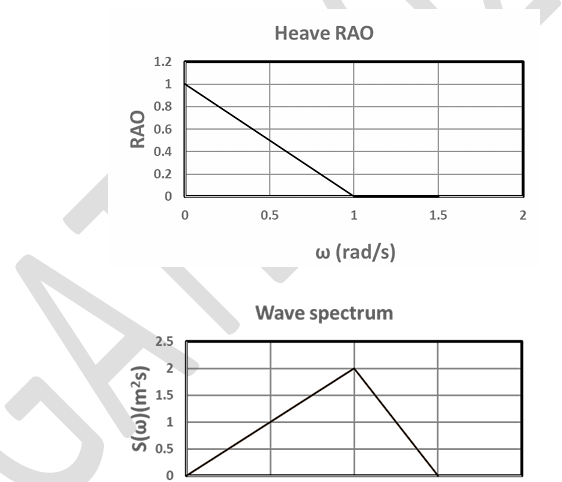
\includegraphics[width=0.5\linewidth]{figures.tex/Screenshot 2025-08-22 152235.png}
    \caption{Caption}
    \label{fig:placeholder}
\end{figure}


  \item
  Consider a thin-walled closed cylindrical steel vessel with an internal pressure of $2~\mathrm{N/mm^2}$. The inner diameter is $1~\mathrm{m}$, and the thickness of the wall is $10~\mathrm{mm}$. The hoop stress is \_\_\_\_\_\_ $~\mathrm{N/mm^2}$ (rounded off to one decimal place).\hfill \textbf{ (GATE NM 2024)}

  \item
  A propeller disc of diameter $2~\mathrm{m}$ produces a thrust of $88~\mathrm{kN}$ while advancing at a speed of $5~\mathrm{m/s}$ in fresh water of density $1000~\mathrm{kg/m^3}$. Based on the axial momentum theory, the propeller efficiency is \_\_\_\_\_\_ \% (rounded off to one decimal place).\hfill \textbf{ (GATE NM 2024)}

  \item
  Consider a rectangular plate with in-plane loads. The state of stress at an arbitrary angle $\theta$ is defined by $\sigma_x$, $\sigma_y$ and $\tau_{xy}$ as shown in the figure. If the principal plane is at $\theta = 45^\circ$, and the principal stresses are $\sigma_x = 8~\mathrm{N/mm^2}$ and $\sigma_y = 3~\mathrm{N/mm^2}$, then the corresponding $\tau_{xy} = \_\_\_\_\_\_~\mathrm{N/mm^2}$.\hfill \textbf{ (GATE NM 2024)}


\begin{figure}
    \centering
    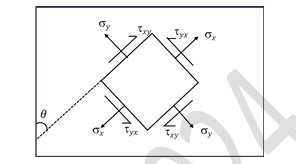
\includegraphics[width=0.5\linewidth]{figures.tex/Screenshot 2025-08-22 153911.png}
    \caption{Caption}
    \label{fig:placeholder}
\end{figure}

\item 
A ship of $5000$ tonnes displacement has a rectangular tank $6~\mathrm{m}$ long and $10~\mathrm{m}$ wide, half-filled with oil of relative density $0.9$. The virtual reduction in the transverse metacentric height of the ship due to free surface effect of the oil in the tank is \_\_\_\_\_\_ cm.\hfill \textbf{ (GATE NM 2024)}

  \item
  An ocean wave of period $8~\mathrm{s}$ and height $2~\mathrm{m}$ is propagating in the Indian Ocean from south to north. According to linear wave theory, for the wave to be considered as a deep-water wave, the minimum water depth should be \_\_\_\_\_\_ m (rounded off to the nearest integer).\hfill \textbf{ (GATE NM 2024)}

  \item
  Consider a gas turbine combustor with air as the working fluid. The flow enters the combustor at $360~\mathrm{K}$ and leaves at $1400~\mathrm{K}$ with a mass flow rate of $1~\mathrm{kg/s}$. The changes in kinetic energy and potential energy of the flow are neglected. Assuming $c_{p,a} = 1.017~\mathrm{kJ/kgK}$ and $c_{p,g} = 1.082~\mathrm{kJ/kgK}$, the heat of combustion is \_\_\_\_\_\_ kW (rounded off to the nearest integer).\hfill \textbf{ (GATE NM 2024)}

  \item
  Consider a circular cylinder of diameter $0.5~\mathrm{m}$ and length $2~\mathrm{m}$, rotating in clockwise direction at a speed of $10~\mathrm{rpm}$ in a flow of velocity $2~\mathrm{m/s}$. Assume the density of fluid is $1250~\mathrm{kg/m^3}$ and $\pi = 3.14$. By Kutta–Joukowski theorem, the lift force on the cylinder is \_\_\_\_\_\_ N (rounded off to the nearest integer).\hfill \textbf{ (GATE NM 2024)}

  \item
  A new absolute temperature scale is proposed based on a Carnot engine operating between hot and cold reservoirs of temperatures $T_h = 7$ and $T_c = 3$ (arbitrary units). Let $Q_h$ and $Q_c$ be the respective heat transfers, with $Q_c = 9$. For consistency with the Kelvin scale, the difference between heats exchanged per cycle must satisfy $\dfrac{Q_h}{Q_c} = \dfrac{T_h}{T_c}$. On the new scale, if the ice point of water is $32^\circ$F and the steam point of water is $212^\circ$F, then the value of ice point of water on this scale is \_\_\_\_\_\_ units (rounded off to the nearest integer).\hfill \textbf{ (GATE NM 2024)}
  
\end{enumerate}

\end{document}
